\documentclass[11pt,a4paper]{article}

\usepackage[utf8]{inputenc}
\usepackage[T1]{fontenc}
\usepackage[brazilian]{babel}
\usepackage{geometry}
\usepackage{graphicx}
\usepackage{booktabs}
\usepackage{amsmath}
\usepackage{float}
\usepackage{hyperref}

\geometry{margin=2.4cm}
\hypersetup{hidelinks}
\setlength{\parskip}{0.45em}
\setlength{\parindent}{0pt}

\title{DBO na entrada com 10 leituras de DQO e SST\\[0.3em]
\large Rede recorrente e validação temporal}
\author{SoftSensor}
\date{16 de outubro de 2026}

\begin{document}
\maketitle

\section{Objetivo}

Estimar a DBO na entrada da estação, \texttt{DBO-E}, guardando 10 leituras de cada entrada. As entradas continuam sendo a DQO (\texttt{DQO-E}) e o SST (\texttt{SS-E}). Cada exemplo é a fila dessas duas medidas no dia estimado e nas nove leituras anteriores disponíveis. A rede lê a fila em ordem e devolve a DBO do dia mais recente.

\section{Dados e janela}

O conjunto é o Water Treatment Plant, de Manel Poch (UCI, 1993). São 527 dias. Ficam 498 dias em que \texttt{DBO-E}, \texttt{DQO-E} e \texttt{SS-E} existem juntos; 29 dias saem por valor ausente. Não há interpolação. As unidades não estão documentadas na UCI.

A fila segue a próxima leitura disponível, não o dia de calendário seguinte. O intervalo mediano entre leituras é 1 dia. Em 116 pares o intervalo passa de um dia, e o maior é de 32 dias. Uma janela de 10 leituras cobre, na mediana, 11 dias de calendário, e no máximo 43.

A série completa vai de 1 de janeiro de 1990 a 29 de outubro de 1991. A DBO média dos dias de treino usados como alvo é 195,02. Nos 100 dias de teste, a partir de 29 de maio de 1991, a média cai para 163,77 e o desvio cai de 65,73 para 36,82.

\section{Protocolo}

Os 398 dias mais antigos treinam. Os 100 mais recentes testam. A divisão é cronológica. Janelas vizinhas compartilham nove leituras, então um sorteio aleatório, como o do MLP anterior, misturaria o futuro com o passado. Surgem 389 janelas de treino, porque as nove primeiras leituras só entram como histórico, e 100 janelas de teste. A primeira janela de teste usa as últimas leituras do treino como histórico; o alvo dela já é um dia de teste.

A validação cruzada fica restrita ao treino e também é temporal (\texttt{TimeSeriesSplit}, 5 partições). O critério é o MAE. Dentro de cada partição, a padronização da DQO, do SST e da DBO usa só as janelas de treino daquela partição.

A rede é uma RNN de Elman: uma camada recorrente com tangente hiperbólica e uma saída linear sobre o estado final. O treino é Adam, com retropropagação no tempo e corte de gradiente. A grade cobre estados de 8, 16 e 32 unidades e taxas de aprendizado \(10^{-3}\) e \(10^{-2}\). O ajuste final repete, em todas as janelas de treino, o número mediano de épocas em que a configuração vencedora parou na validação.

Três referências usam o mesmo corte: a média da DBO de treino, a regressão linear só com a leitura mais recente e a regressão linear com as 10 leituras achatadas.

\section{Resultados}

A validação escolhe estado de 8 unidades e taxa \(10^{-2}\). O MAE nas partições é 42,79, com desvio 3,94. A parada ocorre em 6 épocas. A rede tem 97 parâmetros. As seis configurações ficam entre 42,79 e 45,56 de MAE: aumentar o estado não reduz o erro.

\begin{table}[H]
\centering
\caption{Erro nos 100 dias finais, de 29 de maio a 29 de outubro de 1991.}
\begin{tabular}{lrrr}
\toprule
Modelo & MAE & RMSE & \(R^{2}\) \\
\midrule
Média do treino & 40,88 & 48,15 & $-$0,73 \\
Linear da leitura atual & 33,13 & 40,75 & $-$0,24 \\
Linear das 10 leituras & 34,08 & 42,83 & $-$0,37 \\
RNN & 32,00 & 40,68 & $-$0,23 \\
\bottomrule
\end{tabular}
\end{table}

A reta da leitura atual, neste corte, é
\begin{equation}
\widehat{\mathrm{DBO}} = 73{,}02 + 0{,}3058\,\mathrm{DQO} - 0{,}0139\,\mathrm{SST}.
\end{equation}
Na fila achatada, o coeficiente da DQO do dia estimado é 0,250 e o da DQO anterior é 0,086. Os lags mais antigos de DQO ficam perto de zero. O SST do dia estimado tem coeficiente cerca de zero. A soma dos valores absolutos é 0,432 na DQO e 0,184 no SST.

No teste, a previsão da RNN vai de 109,13 a 266,26, e a DBO observada vai de 84 a 277. O resíduo médio (observado menos previsto) é $-$21,90. A mediana do erro absoluto é 25,87 e o percentil 90 é 57,13. Em 53 dos 100 dias o erro absoluto fica até 30; em 77 dias, até 50.

\begin{figure}[H]
\centering
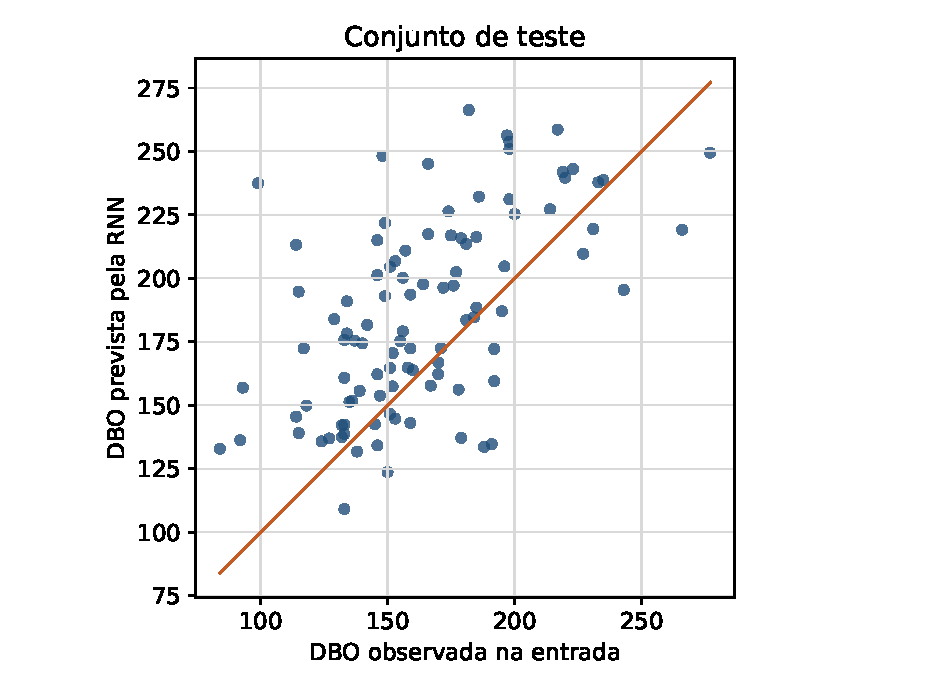
\includegraphics[width=0.72\textwidth]{figuras/rnn_observado_previsto.pdf}
\caption{Teste da RNN. A reta marca a previsão igual à observação. A nuvem fica acima dela: a rede prevê DBO mais alta do que a medida no período final.}
\label{fig:previsto}
\end{figure}

\begin{figure}[H]
\centering
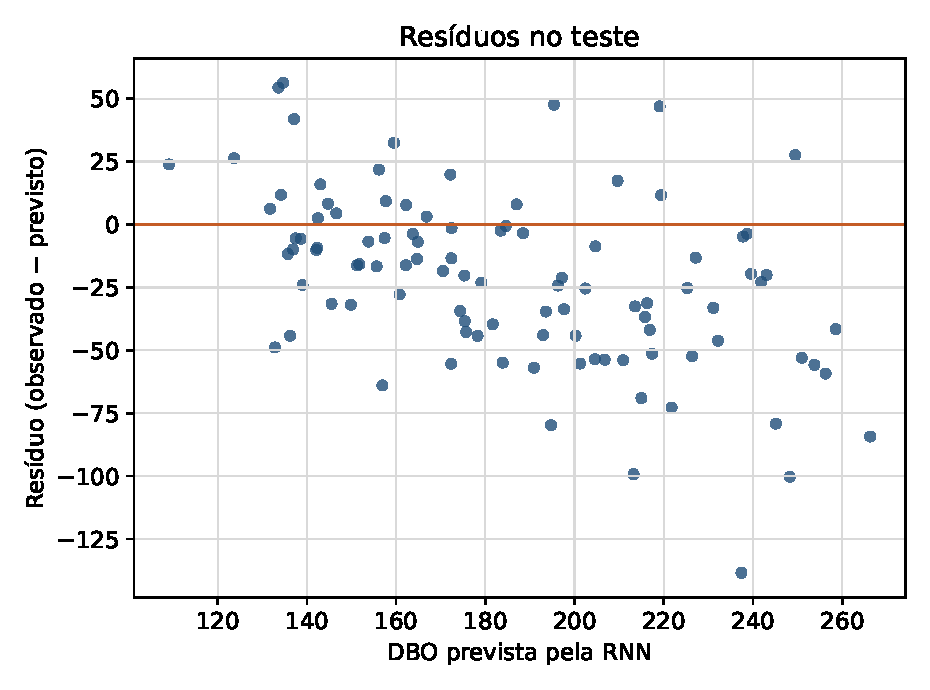
\includegraphics[width=0.72\textwidth]{figuras/rnn_residuos.pdf}
\caption{Resíduos no teste. O centro da nuvem está abaixo de zero, e os maiores desvios aparecem quando a previsão passa de 220.}
\label{fig:residuos}
\end{figure}

\begin{figure}[H]
\centering
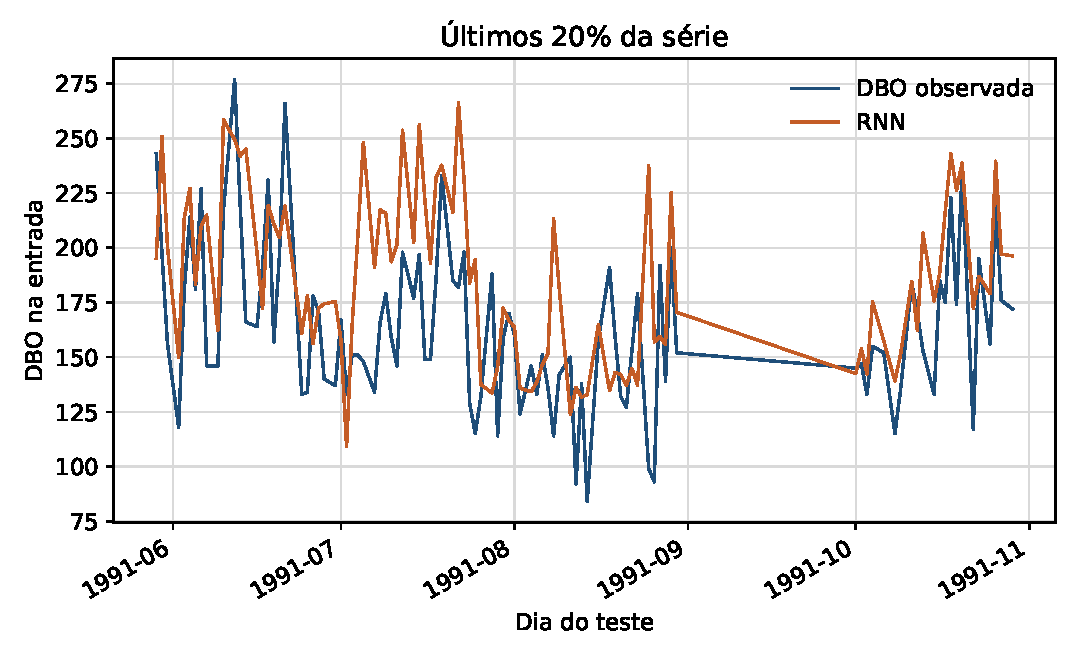
\includegraphics[width=0.92\textwidth]{figuras/rnn_serie.pdf}
\caption{Os 100 dias de teste. A linha liga leituras disponíveis, então um trecho longo e quase reto é um intervalo sem medida, não uma DBO constante.}
\label{fig:serie}
\end{figure}

\section{Leitura}

A RNN reduz o MAE de 40,88 para 32,00 em relação a repetir a média do treino. O \(R^{2}\) de $-$0,23 diz outra coisa: no período de teste, prever a média desse próprio período erraria menos do que a rede. O motivo é o nível. O treino vive em torno de 195 e o teste em torno de 164. A rede, ajustada no primeiro nível, fica em média 22 unidades acima das observações finais. Com desvio de 37 no teste, esse deslocamento domina o \(R^{2}\).

A Figura~\ref{fig:serie} mostra que a forma do dia a dia é em parte acompanhada: picos e vales aparecem nos dois traços. A Figura~\ref{fig:previsto} mostra o deslocamento para cima. A Figura~\ref{fig:residuos} concentra resíduos negativos, em especial nas previsões altas.

A leitura atual, sozinha, chega a MAE 33,13 e RMSE 40,75. A RNN fica em 32,00 e 40,68. A diferença cabe dentro do desvio de 3,94 da validação cruzada. Guardar as nove leituras anteriores não separa a rede da reta de uma leitura.

A linear com as 10 leituras fica atrás da linear de uma leitura (MAE 34,08 e \(R^{2}\) $-$0,37). Os lags antigos têm coeficiente pequeno e sinal instável. No período futuro, esse detalhe do passado aumenta o erro. O estado maior da RNN repete o padrão: 16 e 32 unidades pioram o MAE da validação em relação ao estado de 8.

O sinal que resta é o da DQO recente. O SST, ao longo das 10 leituras, continua sem um efeito estável. A fila de 10 não corrige a queda de nível da DBO entre maio e outubro de 1991, porque DQO e SST desse trecho ainda empurram a previsão para o patamar antigo.

\section{Conclusão}

Com 10 leituras de DQO e de SST, a RNN de 8 unidades chega a MAE 32,00 e RMSE 40,68 nos 100 dias finais, e a \(R^{2}\) $-$0,23. A regressão linear da leitura mais recente fica ao lado, com MAE 33,13 e RMSE 40,75. As leituras anteriores não melhoram a estimativa de forma clara, e o teste cronológico revela uma DBO mais baixa do que a do treino, deslocamento que a fila não absorve.

O notebook é \texttt{modelo/rnn\_dbo\_entrada.ipynb}. O MLP de leituras independentes está em \texttt{docs/mlp\_dbo\_entrada.pdf}; o corte daquele relatório é aleatório, e os \(R^{2}\) dos dois documentos não se comparam direto.
\end{document}
